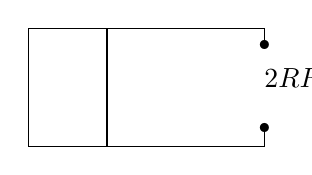
\begin{tikzpicture}[
	font=\footnotesize,
	]
	\draw (0,15pt)node{$\bullet$}node[right]{\ptA}|-(-3,.75)--++(0,-1.5)-|(0,-15pt)node{$\bullet$}node[right]{\ptB};
	\draw (-2,-.75)--++(0,1.5);
	\resistanceV{shift={(-3,0)}}{$2R$};
	\resistanceV{shift={(-2,0)}}{$R'$};
	\resistanceH{shift={(-1,.75)}}{$R$};
	\resistanceH{shift={(-1,-.75)}}{$R$};
\end{tikzpicture}